\chapter{Θεωρητικό Μέρος}

\section{Κυβερνοασφάλεια στα Δίκτυα \en{5G} και \en{6G}}


Η ταχεία εξέλιξη των κινητών δικτύων προς το \en{5G} και το επερχόμενο \en{6G} έχει εισαγάγει πρωτοφανείς δυνατότητες όσον αφορά τη συνδεσιμότητα,
την ταχύτητα και τη νοημοσύνη. Ωστόσο, αυτός ο μετασχηματισμός έχει αυξήσει σημαντικά την πολυπλοκότητα των υποδομών δικτύου, 
οδηγώντας σε νέες προκλήσεις κυβερνοασφάλειας. Σε αντίθεση με τις προηγούμενες γενιές, τα δίκτυα επόμενης γενιάς βασίζονται σε μεγάλο βαθμό
 σε \en{software-defined} στοιχεία, εικονικοποίηση και κατανεμημένες αρχιτεκτονικές, τα οποία διευρύνουν την επιφάνεια επίθεσης.

Η κυβερνοασφάλεια στα δίκτυα \en{5G} και \en{6G} δεν αποτελεί απλώς επέκταση της παραδοσιακής ασφάλειας δικτύων, αλλά απαιτεί μια θεμελιωδώς νέα προσέγγιση 
που ενσωματώνει παρακολούθηση σε πραγματικό χρόνο, ευφυή ανίχνευση απειλών και αυτοματοποιημένους μηχανισμούς απόκρισης \cite{ferrag2019security}. 
Το κεφάλαιο αυτό εξετάζει τους κύριους τύπους κυβερνοαπειλών, τους παράγοντες που συμβάλλουν στη διεύρυνση της επιφάνειας επίθεσης και την ανάγκη για προηγμένες 
λύσεις ασφάλειας.

\subsection{Τύποι Κυβερνοαπειλών}

\subsubsection{Επιθέσεις \en{Distributed Denial of Service (DDoS)}}

Οι επιθέσεις \en{Distributed Denial of Service (DDoS)} παραμένουν μία από τις πιο διαδεδομένες απειλές στα σύγχρονα δίκτυα. Στόχος τους είναι η υπερφόρτωση των πόρων του δικτύου μέσω τεράστιου όγκου κίνησης, καθιστώντας τις υπηρεσίες μη διαθέσιμες στους νόμιμους χρήστες. Στα περιβάλλοντα \en{5G}, το υψηλό εύρος ζώνης και η μαζική συνδεσιμότητα μπορούν να ενισχύσουν τον αντίκτυπο τέτοιων επιθέσεων \cite{zhang2019ddos}. Η ενσωμάτωση συσκευών \en{IoT} επιδεινώνει περαιτέρω το πρόβλημα, καθώς παραβιασμένες συσκευές μπορούν να σχηματίσουν μεγάλα \en{botnets}. Στο \en{6G}, η κλίμακα αυτών των επιθέσεων αναμένεται να αυξηθεί σημαντικά.

\subsubsection{Επιθέσεις Εισβολής και \en{Malware}}

Οι επιθέσεις εισβολής και \en{malware} στοχεύουν την υποδομή του δικτύου και τις συσκευές χρηστών για μη εξουσιοδοτημένη πρόσβαση ή κλοπή δεδομένων. Στα δίκτυα \en{5G}, η χρήση εικονικοποίησης και \en{cloud-native} τεχνολογιών εισάγει νέες ευπάθειες, καθώς οι επιτιθέμενοι μπορούν να εκμεταλλευτούν σφάλματα λογισμικού ή λανθασμένες ρυθμίσεις σε \en{virtual network functions (VNFs)} \cite{ahmed2020survey}. Ιδιαίτερη ανησυχία προκαλούν επίσης, τα \en{advanced persistent threats (APTs)}, τα οποία παραμένουν σε ένα σύστημα για μεγάλο χρονικό διάστημα καθώς η έγκαιρη ανίχνευσή τους είναι δύσκολη.

\subsubsection{Επιθέσεις Σηματοδοσίας}

Οι επιθέσεις σηματοδοσίας εκμεταλλεύονται ευπάθειες στο επίπεδο ελέγχου των δικτύων. Δημιουργούν υπερβολικό όγκο σημάτων, υπερφορτώνοντας στοιχεία όπως το \en{Mobility Management Entity (MME)} ή το \en{Access and Mobility Management Function (AMF)} \cite{li2018signaling}. Στα δίκτυα \en{5G}, η αρχιτεκτονική βασισμένη σε υπηρεσίες αυξάνει τις πιθανότητες εκμετάλλευσης τέτοιων αδυναμιών.

\subsubsection{Παραβιάσεις και Διαρροές Δεδομένων}

Οι παραβιάσεις και διαρροές δεδομένων αποτελούν σοβαρή απειλή, καθώς τεράστιοι όγκοι ευαίσθητων πληροφοριών μεταδίδονται και επεξεργάζονται. Η μη εξουσιοδοτημένη πρόσβαση μπορεί να έχει σοβαρές συνέπειες \cite{roman2018mobile}. Η κατανεμημένη φύση των δικτύων \en{5G}/\en{6G}, σε συνδυασμό με \en{edge computing} και υποδομές \en{cloud}, αυξάνει τα πιθανά σημεία επίθεσης.

\subsection{Διευρυμένη Επιφάνεια Επίθεσης}

Η διευρυμένη επιφάνεια επίθεσης στα σύγχρονα δίκτυα οφείλεται σε πολλαπλούς τεχνολογικούς παράγοντες. Η εξάπλωση του \en{Internet of Things (IoT)} αποτελεί έναν από τους σημαντικότερους, καθώς οι συσκευές αυτές συχνά στερούνται ισχυρών μηχανισμών ασφάλειας και προστασίας \cite{atzori2010internet}. Παράλληλα, ο τεράστιος αριθμός τους αυξάνει σημαντικά την πιθανότητα εκμετάλλευσης ευπαθειών και τη δημιουργία κακόβουλων δικτύων \en{botnets}. Επιπλέον, η υιοθέτηση τεχνολογιών όπως \en{Network Function Virtualization (NFV)} και \en{Software-Defined Networking (SDN)} εισάγει νέες προκλήσεις ασφάλειας \cite{kreutz2015software}. Ευπάθειες σε \en{hypervisors}, εικονικές μηχανές ή πλατφόρμες ορχήστρωσης μπορούν να επηρεάσουν ταυτόχρονα πολλαπλές λειτουργίες του δικτύου, αυξάνοντας τον συνολικό κίνδυνο και την πολυπλοκότητα της προστασίας.

\subsection{Ανάγκη για Ανίχνευση και Απόκριση σε Πραγματικό Χρόνο}

Λόγω της πολυπλοκότητας των σύγχρονων δικτύων, οι παραδοσιακές προσεγγίσεις ασφάλειας δεν επαρκούν πλέον. Απαιτούνται μηχανισμοί ανίχνευσης και απόκρισης σε πραγματικό χρόνο. Τεχνολογίες όπως η μηχανική μάθηση και το \en{AI} χρησιμοποιούνται για την ανάλυση μεγάλων όγκων δεδομένων και τον εντοπισμό ανωμαλιών \cite{nguyen2018deep,ilias2025convolutional}. Οι σύγχρονες λύσεις πρέπει να μπορούν να:
\begin{itemize}
    \item Αναγνωρίζουν κακόβουλα πρότυπα συμπεριφοράς
    \item Αντιδρούν αυτόματα σε απειλές
    \item Προσαρμόζονται σε εξελισσόμενες επιθέσεις
\end{itemize}

\section{Αρχεία Καταγραφής Δικτύου και Ασφάλεια}

\subsection{Εισαγωγή}

Τα αρχεία καταγραφής δικτύου αποτελούν θεμελιώδη πηγή πληροφορίας για την παρακολούθηση, διαχείριση και ασφάλεια των σύγχρονων συστημάτων επικοινωνίας. Στο πλαίσιο των δικτύων \en{5G} και του αναδυόμενου \en{6G}, όπου οι υποδομές είναι ιδιαίτερα δυναμικές, κατανεμημένες και βασισμένες σε λογισμικό, η σημασία των αρχείων καταγραφής έχει αυξηθεί σημαντικά. Τα αρχεία αυτά παρέχουν λεπτομερείς καταγραφές συμβάντων συστήματος, δραστηριοτήτων χρηστών και συμπεριφοράς δικτύου, επιτρέποντας στους διαχειριστές και στους μηχανισμούς ασφάλειας να εντοπίζουν ανωμαλίες, να διαγιγνώσκουν προβλήματα και να ανταποκρίνονται σε κυβερνοαπειλές.

Λόγω της πολυπλοκότητας και της κλίμακας των δικτύων επόμενης γενιάς, τα δεδομένα καταγραφής παράγονται με πρωτοφανή ρυθμό. Ως εκ τούτου, η αποτελεσματική ανάλυσή τους αποτελεί σημαντική πρόκληση, απαιτώντας προηγμένα εργαλεία και τεχνικές όπως η ανάλυση \en{big data} και η μηχανική μάθηση \cite{behl2017cybersecurity}. Το κεφάλαιο αυτό εξετάζει τους τύπους αρχείων καταγραφής, τα χαρακτηριστικά τους και τις προκλήσεις που σχετίζονται με την ανάλυσή τους.

\subsection{Ορισμός και Τύποι Αρχείων Καταγραφής Δικτύου}

Τα αρχεία καταγραφής δικτύου είναι δομημένες ή μη δομημένες εγγραφές που δημιουργούνται από συσκευές, εφαρμογές και συστήματα δικτύου και καταγράφουν γεγονότα που συμβαίνουν εντός του δικτύου. Είναι απαραίτητα για τον έλεγχο, την αντιμετώπιση προβλημάτων και την παρακολούθηση ασφάλειας.

\subsubsection{Αρχεία Καταγραφής Συστήματος}

Τα αρχεία καταγραφής συστήματος καταγράφουν γεγονότα που σχετίζονται με τη λειτουργία των συσκευών του δικτύου. Περιλαμβάνουν πληροφορίες για την εκκίνηση και τον τερματισμό του συστήματος, πιθανές αλλαγές στις ρυθμίσεις, μηνύματα σφαλμάτων και χρήση πόρων. Στα περιβάλλοντα \en{5G}/\en{6G}, δημιουργούνται από διάφορα στοιχεία όπως σταθμοί βάσης, λειτουργίες δικτύου κορμού και στοιχεία εικονικοποιημένης υποδομής. Είναι ιδιαίτερα χρήσιμα για τον εντοπισμό βλαβών και μη εξουσιοδοτημένων αλλαγών, καθώς και για την ψηφιακή διερεύνηση περιστατικών ασφάλειας \cite{xu2009detecting}.

\subsubsection{Αρχεία Καταγραφής Κίνησης}

Τα αρχεία καταγραφής κίνησης περιλαμβάνουν πληροφορίες σχετικά με τα πακέτα δεδομένων που μεταδίδονται στο δίκτυο. Συνήθως περιλαμβάνουν διευθύνσεις \en{IP}, αριθμούς θυρών, πρωτόκολλα, μεγέθη πακέτων και χρονικές σφραγίδες. Είναι κρίσιμα για την κατανόηση της συμπεριφοράς του δικτύου και τον εντοπισμό ύποπτων προτύπων. Στα δίκτυα επόμενης γενιάς, δημιουργούνται σε πολλαπλά επίπεδα, συμπεριλαμβανομένων του \en{RAN}, του πυρήνα και των κόμβων \en{edge computing} \cite{garcia2014anomaly}.

\subsubsection{Αρχεία Καταγραφής Πρόσβασης}

Τα αρχεία καταγραφής πρόσβασης παρακολουθούν δραστηριότητες ταυτοποίησης και εξουσιοδότησης χρηστών. Καταγράφουν προσπάθειες σύνδεσης, επιτυχείς ή αποτυχημένες εισόδους στο σύστημα και διάρκεια συνδέσεων. Είναι κρίσιμα για τον εντοπισμό μη εξουσιοδοτημένης πρόσβασης και εσωτερικών απειλών, ιδιαίτερα στα δίκτυα \en{5G}/\en{6G} με μεγάλο αριθμό συσκευών \cite{scarfone2007guide}.

\subsection{Χαρακτηριστικά των Αρχείων Καταγραφής}

Τα αρχεία καταγραφής (\en{log files}) παρουσιάζουν ιδιαίτερα χαρακτηριστικά που δημιουργούν σημαντικές προκλήσεις κατά την αποθήκευση, επεξεργασία και ανάλυσή τους. Ένα από τα βασικότερα χαρακτηριστικά είναι ο μεγάλος όγκος δεδομένων που παράγεται καθημερινά από εκατομμύρια συνδεδεμένες συσκευές, γεγονός που απαιτεί κλιμακούμενες λύσεις αποθήκευσης και επεξεργασίας, όπως τα \en{Hadoop} και \en{Apache Spark} \cite{behl2017cybersecurity}. Επιπλέον, τα δεδομένα καταγραφής παράγονται με ιδιαίτερα υψηλή ταχύτητα και συχνά απαιτούν επεξεργασία σε πραγματικό χρόνο, ειδικά σε εφαρμογές κυβερνοασφάλειας και ανίχνευσης απειλών, όπου τεχνολογίες όπως το \en{Apache Kafka} και συστήματα ανίχνευσης εισβολών σε πραγματικό χρόνο χρησιμοποιούνται για την αποτελεσματική διαχείρισή τους \cite{chen2014big}. Παράλληλα, ένα ακόμη σημαντικό χαρακτηριστικό είναι η μη δομημένη ή ημι-δομημένη φύση των δεδομένων αυτών, καθώς τα αρχεία καταγραφής μπορεί να εμφανίζονται σε διαφορετικές μορφές, όπως \en{JSON}, \en{syslog} ή ακόμη και ως ελεύθερο κείμενο. Η έλλειψη ενιαίας μορφοποίησης δυσκολεύει σημαντικά τη διαδικασία ανάλυσης και απαιτεί τη χρήση τεχνικών όπως η κανονικοποίηση δεδομένων και η επεξεργασία φυσικής γλώσσας (\en{Natural Language Processing - NLP}) \cite{he2017drain}.

\subsection{Προκλήσεις στην Ανάλυση Αρχείων Καταγραφής}

Η ανάλυση αρχείων καταγραφής συνοδεύεται από σημαντικές προκλήσεις που σχετίζονται με τον όγκο, την ποιότητα και την πολυπλοκότητα των δεδομένων. Τα αρχεία καταγραφής περιέχουν συχνά θόρυβο, άσχετες πληροφορίες ή επαναλαμβανόμενα γεγονότα, γεγονός που δυσκολεύει την εξαγωγή χρήσιμων συμπερασμάτων και την έγκαιρη ανίχνευση περιστατικών ασφαλείας. Για την αντιμετώπιση αυτού του προβλήματος χρησιμοποιούνται τεχνικές όπως \en{log aggregation}, αποδιπλοποίηση και ανίχνευση ανωμαλιών \cite{xu2009detecting}. Επιπλέον, λόγω του τεράστιου όγκου και της αυξημένης πολυπλοκότητας των δεδομένων, η χειροκίνητη ανάλυση δεν θεωρείται πλέον εφικτή ή αποδοτική. Ως αποτέλεσμα, απαιτούνται αυτοματοποιημένες προσεγγίσεις, όπως η μηχανική μάθηση και η εξόρυξη δεδομένων, για τον εντοπισμό προτύπων, αποκλίσεων και πιθανών απειλών \cite{garcia2014anomaly}.

\subsection{Ρόλος των Αρχείων Καταγραφής στην Ασφάλεια}

Τα αρχεία καταγραφής παίζουν κεντρικό ρόλο στην ασφάλεια των δικτύων \en{5G} και \en{6G}. Παρέχουν τα απαραίτητα δεδομένα για συστήματα ανίχνευσης εισβολών, πλατφόρμες \en{security information and event management (SIEM)} και εγκληματολογικές αναλύσεις.

Μέσω της ανάλυσής τους μπορούν να:
\begin{itemize}
    \item Ανιχνεύσουν ανώμαλη συμπεριφορά
    \item Εντοπίσουν κυβερνοεπιθέσεις
    \item Εντοπίσουν την προέλευση περιστατικών ασφάλειας
    \item Παρακολουθούν τη συμμόρφωση με πολιτικές ασφάλειας
\end{itemize}

Στα δίκτυα επόμενης γενιάς, η ενσωμάτωση \en{AI} και αναλύσεων \en{big data} αναμένεται να ενισχύσει περαιτέρω τη σημασία τους.

\section{Παραδοσιακές Προσεγγίσεις στην Ανάλυση Αρχείων Καταγραφής}

\subsection{Εισαγωγή}

Η ανάλυση αρχείων καταγραφής αποτελεί διαχρονικά βασικό πυλώνα της ασφάλειας δικτύων, επιτρέποντας την ανίχνευση ανωμαλιών, εισβολών και σφαλμάτων συστήματος. Πριν την εμφάνιση των σύγχρονων τεχνικών βαθιάς μάθησης, οι παραδοσιακές προσεγγίσεις βασίζονταν σε συστήματα βασισμένα σε κανόνες, ανίχνευση βάσει υπογραφών και κλασικές μεθόδους μηχανικής μάθησης. Οι τεχνικές αυτές έχουν υιοθετηθεί ευρέως σε συστήματα \en{Security Information and Event Management (SIEM)} και \en{intrusion detection systems (IDS)}, αποτελώντας τη βάση πολλών υπαρχουσών λύσεων κυβερνοασφάλειας.

Παρά την αποτελεσματικότητά τους σε ορισμένα σενάρια, οι παραδοσιακές μέθοδοι παρουσιάζουν σημαντικούς περιορισμούς όταν εφαρμόζονται σε σύγχρονα περιβάλλοντα \en{5G} και \en{6G}. Ο αυξανόμενος όγκος, η ταχύτητα και η πολυπλοκότητα των δεδομένων απαιτούν πιο επεκτάσιμες και προσαρμοστικές λύσεις. Το κεφάλαιο αυτό εξετάζει τις βασικές παραδοσιακές προσεγγίσεις και τους περιορισμούς τους.

\subsection{Συστήματα Βασισμένα σε Κανόνες}

Τα συστήματα βασισμένα σε κανόνες αποτελούν μία από τις πρώτες και πιο διαδεδομένες προσεγγίσεις για την ανάλυση αρχείων καταγραφής. Βασίζονται σε προκαθορισμένους κανόνες που περιγράφουν γνωστά πρότυπα κακόβουλης ή ανώμαλης συμπεριφοράς. Οι αναλυτές ασφάλειας ορίζουν αυτούς τους κανόνες χειροκίνητα. Τα συστήματα \en{SIEM} αποτελούν χαρακτηριστικό παράδειγμα. Συλλέγουν και συσχετίζουν δεδομένα καταγραφής από πολλαπλές πηγές και εφαρμόζουν κανόνες συσχέτισης για την ανίχνευση συμβάντων ασφάλειας \cite{behl2017cybersecurity}. Παρότι είναι εύκολα στην υλοποίηση και ερμηνεύσιμα, εξαρτώνται από χειροκίνητη συντήρηση και αδυνατούν να ανιχνεύσουν νέες ή εξελισσόμενες απειλές.

\subsection{Ανίχνευση Βάσει Υπογραφών}

Η ανίχνευση βάσει υπογραφών χρησιμοποιείται ευρέως σε συστήματα ανίχνευσης εισβολών και λογισμικά προστασίας από ιούς. Αναγνωρίζει απειλές συγκρίνοντας μοτίβα με μια βάση γνωστών υπογραφών \cite{garcia2009anomaly}. Το βασικό πλεονέκτημα είναι η υψηλή ακρίβεια για γνωστές απειλές με χαμηλές ψευδώς θετικές προβλέψεις. Ωστόσο, είναι αναποτελεσματική έναντι επιθέσεων μηδενικής ημέρας (\en{zero-day}) και άγνωστων απειλών. Σε σύγχρονα δίκτυα, όπου οι επιθέσεις εξελίσσονται συνεχώς, απαιτούνται συχνές ενημερώσεις των βάσεων υπογραφών.

\subsection{Προσεγγίσεις Μηχανικής Μάθησης}

Για την αντιμετώπιση των περιορισμών των προηγούμενων μεθόδων, έχουν αναπτυχθεί τεχνικές μηχανικής μάθησης (\en{ML}).

\subsubsection{Επιβλεπόμενη Μάθηση}

Οι μέθοδοι επιβλεπόμενης μάθησης χρησιμοποιούν επισημασμένα δεδομένα για την εκπαίδευση μοντέλων που ταξινομούν συμβάντα ως κανονικά ή κακόβουλα. Συνήθεις αλγόριθμοι περιλαμβάνουν δέντρα αποφάσεων, \en{support vector machines (SVM)} και νευρωνικά δίκτυα \cite{nguyen2018deep}. Παρουσιάζουν υψηλή ακρίβεια όταν υπάρχουν επαρκή δεδομένα, αλλά η συλλογή επισημασμένων δεδομένων είναι δύσκολη και δεν γενικεύονται εύκολα σε νέες επιθέσεις.

\subsubsection{Μη Επιβλεπόμενη Μάθηση}

Οι τεχνικές μη επιβλεπόμενης μάθησης δεν απαιτούν επισημασμένα δεδομένα. Εντοπίζουν πρότυπα και ανωμαλίες μέσω αλγορίθμων όπως το \en{k-means} \cite{garcia2009anomaly}. Είναι χρήσιμες για τον εντοπισμό άγνωστων επιθέσεων, αλλά συχνά παράγουν πολλά ψευδώς θετικά και απαιτούν επιπλέον ανάλυση.

\subsection{Περιορισμοί Παραδοσιακών Προσεγγίσεων}

Οι παραδοσιακές προσεγγίσεις παρουσιάζουν σημαντικούς περιορισμούς ως προς την εφαρμογή τους σε σύγχρονα δίκτυα μεγάλης κλίμακας. Αρχικά, εμφανίζουν περιορισμένη επεκτασιμότητα, καθώς δεν κλιμακώνονται εύκολα σε μεγάλα περιβάλλοντα και η επεξεργασία τεράστιου όγκου δεδομένων είναι ιδιαίτερα απαιτητική υπολογιστικά, ειδικά σε δίκτυα όπως το \en{5G}. Επιπλέον, βασίζονται σε μεγάλο βαθμό σε χειροκίνητη επιλογή χαρακτηριστικών (\en{feature engineering}), διαδικασία που απαιτεί εξειδικευμένη γνώση, σημαντικό χρόνο και συνεχή προσαρμογή \cite{he2017drain}. Τέλος, διαθέτουν περιορισμένη ικανότητα γενίκευσης, καθώς δυσκολεύονται να προσαρμοστούν σε νέες ή άγνωστες επιθέσεις, λειτουργώντας κυρίως αντιδραστικά και χωρίς να προσφέρουν επαρκή προστασία απέναντι σε προηγμένες απειλές.

\section{Εισαγωγή στα Μεγάλα Γλωσσικά Μοντέλα (\en{LLMs})}

\subsection{Εισαγωγή}

Τα Μεγάλα Γλωσσικά Μοντέλα (\en{LLMs}) έχουν αναδειχθεί σε μια τεχνολογία που αλλάζει ριζικά τον χώρο της τεχνητής νοημοσύνης, ιδιαίτερα στον τομέα της επεξεργασίας φυσικής γλώσσας (\en{NLP}). Τα μοντέλα αυτά μπορούν να κατανοούν, να παράγουν και να επεξεργάζονται την ανθρώπινη γλώσσα με εντυπωσιακή ακρίβεια. Η επίδρασή τους εκτείνεται σε πολλούς τομείς, όπως η παραγωγή κειμένου, η απάντηση ερωτήσεων, η παραγωγή κώδικα και πιο πρόσφατα, εφαρμογές κυβερνοασφάλειας, όπως η ανάλυση αρχείων καταγραφής και η ανίχνευση ανωμαλιών. Η γρήγορη εξέλιξη των \en{LLMs} έχει γίνει δυνατή χάρη στη διαθεσιμότητα συνόλων δεδομένων μεγάλης κλίμακας, στην αυξημένη υπολογιστική ισχύ και στην ανάπτυξη νέων αρχιτεκτονικών νευρωνικών δικτύων, κυρίως του μοντέλου \en{Transformer} \cite{vaswani2017attention}.

\subsection{Ορισμός των Μεγάλων Γλωσσικών Μοντέλων (\en{LLMs})}

Τα \en{LLMs} είναι μοντέλα βαθιάς μάθησης που εκπαιδεύονται σε τεράστιες ποσότητες κειμενικών δεδομένων, ώστε να μαθαίνουν τη στατιστική δομή της γλώσσας. Συνήθως αποτελούνται από δισεκατομμύρια ή ακόμη και τρισεκατομμύρια παραμέτρους, γεγονός που τους επιτρέπει να αποτυπώνουν σύνθετα γλωσσικά μοτίβα και σχέσεις που εξαρτώνται από τα συμφραζόμενα.

Τα \en{LLMs} λειτουργούν προβλέποντας την πιθανότητα μιας ακολουθίας λέξεων, με βάση το προηγούμενο συμφραζόμενο. Αυτή η ικανότητα τους επιτρέπει να εκτελούν ένα ευρύ φάσμα γλωσσικών εργασιών χωρίς να απαιτείται προγραμματισμός ειδικά για κάθε εργασία. Αντί γι’ αυτό, βασίζονται σε αναπαραστάσεις που έχουν μάθει μέσω προεκπαίδευσης σε ποικίλα σύνολα δεδομένων \cite{brown2020language}.

Τα βασικά χαρακτηριστικά των \en{LLMs} περιλαμβάνουν:
\begin{itemize}
\item Δεδομένα εκπαίδευσης μεγάλης κλίμακας
\item Υψηλή πολυπλοκότητα μοντέλου (εκατομμύρια έως δισεκατομμύρια παράμετροι)
\item Εφαρμοσιμότητα γενικού σκοπού σε διαφορετικές εργασίες
\item Κατανόηση γλώσσας με βάση τα συμφραζόμενα
\end{itemize}

Αυτά τα χαρακτηριστικά καθιστούν τα \en{LLMs} κατάλληλα για την ανάλυση μη δομημένων δεδομένων, όπως τα αρχεία καταγραφής δικτύου, όπου οι παραδοσιακές μέθοδοι συχνά δυσκολεύονται.

\subsection{Αρχιτεκτονική \en{Transformer}}

Η αρχιτεκτονική \en{Transformer}, η οποία παρουσιάστηκε από τους \en{Vaswani et al.} \cite{vaswani2017attention}, αποτελεί το βασικό δομικό στοιχείο των περισσότερων σύγχρονων \en{LLMs}. Σε αντίθεση με παλαιότερα μοντέλα ακολουθιών, όπως τα αναδρομικά νευρωνικά δίκτυα (\en{RNNs}), οι \en{Transformers} βασίζονται αποκλειστικά σε μηχανισμούς προσοχής για την επεξεργασία των δεδομένων εισόδου.

Σε γενικό επίπεδο, ο \en{Transformer} αποτελείται από δομή \en{encoder-decoder}, αν και πολλά \en{LLMs} χρησιμοποιούν μόνο ένα από αυτά τα δύο μέρη, ανάλογα με την εργασία. Η βασική καινοτομία του \en{Transformer} είναι ο μηχανισμός αυτοπροσοχής, ο οποίος επιτρέπει στο μοντέλο να σταθμίζει τη σημασία διαφορετικών λέξεων μέσα σε μια ακολουθία κατά τη δημιουργία αναπαραστάσεων.

Η αυτοπροσοχή υπολογίζει ταυτόχρονα τις σχέσεις μεταξύ όλων των \en{tokens} σε μια ακολουθία, επιτρέποντας στο μοντέλο να αποτυπώνει μακρινές εξαρτήσεις πιο αποτελεσματικά από τα παραδοσιακά μοντέλα. Αυτή η δυνατότητα παράλληλης επεξεργασίας βελτιώνει επίσης σημαντικά την αποδοτικότητα της εκπαίδευσης.

Τα κύρια συστατικά του \en{Transformer} περιλαμβάνουν:
\begin{itemize}
    \item Επίπεδα πολυκέφαλης αυτοπροσοχής (\en{multi-head self-attention layers})
    \item Νευρωνικά δίκτυα πρόσθιας τροφοδότησης (\en{feed-forward neural networks})
    \item Θεσιακή κωδικοποίηση (\en{positional encoding}) για τη διατήρηση της σειράς της ακολουθίας
    \item Κανονικοποίηση επιπέδων (\en{layer normalization}) και υπολειμματικές συνδέσεις (\en{residual connections})
\end{itemize}

Τα στοιχεία αυτά συνεργάζονται για να παράγουν ενσωματώσεις με βάση τα συμφραζόμενα, οι οποίες κωδικοποιούν τόσο τη σημασία των μεμονωμένων λέξεων όσο και τις σχέσεις τους μέσα στην ακολουθία.

\begin{figure}[H]                                                                             
    \centering                                                                                 
    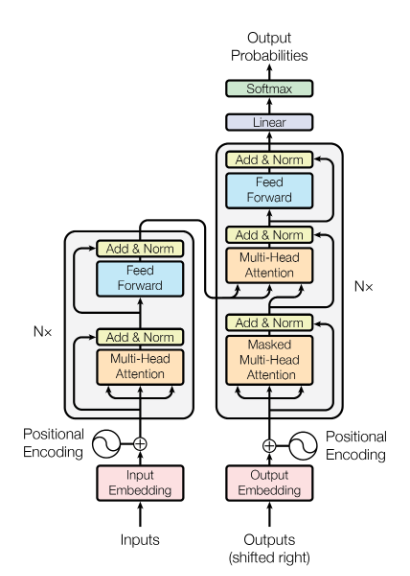
\includegraphics[width=0.5\textwidth]{figures/transformer.png}                              
    \caption{\en{The Transformer - model architecture. Adapted from \cite{vaswani2017attention}.}}                                           
    \label{fig:transformer-architecture}                                                                     
\end{figure}

\subsection{Προεκπαίδευση και Λεπτομερής Προσαρμογή}

Η επιτυχία των \en{LLMs} εξαρτάται σε μεγάλο βαθμό από τη μεθοδολογία εκπαίδευσής τους, η οποία συνήθως περιλαμβάνει δύο βασικά στάδια: την προεκπαίδευση και τη λεπτομερή προσαρμογή.

\subsubsection{Προεκπαίδευση}

Κατά την προεκπαίδευση, το μοντέλο εκπαιδεύεται σε μεγάλης κλίμακας, μη επισημασμένα κείμενα, χρησιμοποιώντας στόχους αυτοεποπτευόμενης μάθησης. Συνηθισμένες εργασίες προεκπαίδευσης περιλαμβάνουν τη γλωσσική μοντελοποίηση (πρόβλεψη της επόμενης λέξης σε μια ακολουθία) και τη μοντελοποίηση γλώσσας με μάσκα (πρόβλεψη λέξεων που λείπουν από μια πρόταση).

Αυτή η φάση επιτρέπει στο μοντέλο να μάθει γενική γλωσσική γνώση, όπως γραμματική, σύνταξη και σημασιολογικές σχέσεις. Επειδή η προεκπαίδευση δεν απαιτεί επισημασμένα δεδομένα, μπορεί να αξιοποιήσει τεράστιες ποσότητες δημόσια διαθέσιμου κειμένου \cite{devlin2019bert}.

\subsubsection{Λεπτομερής Προσαρμογή}

Μετά την προεκπαίδευση, το μοντέλο μπορεί να προσαρμοστεί λεπτομερώς σε ένα μικρότερο σύνολο δεδομένων, ειδικό για μια συγκεκριμένη εργασία. Η λεπτομερής προσαρμογή περιλαμβάνει τη ρύθμιση των παραμέτρων του μοντέλου, ώστε να βελτιστοποιηθεί η απόδοσή του για μια συγκεκριμένη εφαρμογή, όπως η ταξινόμηση, η απάντηση ερωτήσεων ή η ανίχνευση ανωμαλιών.

Η λεπτομερής προσαρμογή επιτρέπει στα \en{LLMs} να προσαρμόζονται σε συγκεκριμένους τομείς, συμπεριλαμβανομένης της κυβερνοασφάλειας, όπου μπορούν να εκπαιδευτούν ώστε να εντοπίζουν μοτίβα σε αρχεία καταγραφής δικτύου ή να ανιχνεύουν ύποπτες δραστηριότητες. Αυτή η διαδικασία εκπαίδευσης δύο σταδίων μειώνει σημαντικά την ανάγκη για μεγάλα επισημασμένα σύνολα δεδομένων σε μεταγενέστερες εργασίες.

\subsection{Παραδείγματα Μεγάλων Γλωσσικών Μοντέλων}

\subsubsection{\en{GPT} (\en{Generative Pre-trained Transformer})}

Η οικογένεια μοντέλων \en{Generative Pre-trained Transformer} (\en{GPT}) αποτελεί χαρακτηριστικό παράδειγμα \en{LLMs} που βασίζονται στην αρχιτεκτονική αποκωδικοποιητή \en{Transformer}. Τα μοντέλα \en{GPT} εκπαιδεύονται χρησιμοποιώντας έναν αυτοπαλίνδρομο στόχο γλωσσικής μοντελοποίησης, όπου το μοντέλο προβλέπει το επόμενο \en{token} σε μια ακολουθία με βάση το προηγούμενο συμφραζόμενο \cite{brown2020language}.

Τα μοντέλα \en{GPT} είναι ιδιαίτερα κατάλληλα για εργασίες παραγωγής κειμένου, όπως συστήματα διαλόγου, δημιουργία περιεχομένου και παραγωγή κώδικα. Η ικανότητά τους να παράγουν συνεκτικό και συναφές ως προς τα συμφραζόμενα κείμενο έχει οδηγήσει στην ευρεία υιοθέτησή τους τόσο στην ακαδημαϊκή κοινότητα όσο και στη βιομηχανία.

\subsubsection{\en{BERT} (\en{Bidirectional Encoder Representations from Transformers})}

Το \en{BERT} είναι ένα ακόμη σημαντικό \en{LLM}, βασισμένο στην αρχιτεκτονική κωδικοποιητή \en{Transformer}. Σε αντίθεση με το \en{GPT}, το οποίο επεξεργάζεται το κείμενο με μονοκατευθυντικό τρόπο, το \en{BERT} χρησιμοποιεί αμφίδρομο συμφραζόμενο, επιτρέποντάς του να λαμβάνει υπόψη τόσο τις προηγούμενες όσο και τις επόμενες λέξεις κατά τη δημιουργία αναπαραστάσεων \cite{devlin2019bert}.

Το \en{BERT} εκπαιδεύεται με τη χρήση μοντελοποίησης γλώσσας με μάσκα και εργασιών πρόβλεψης επόμενης πρότασης, γεγονός που το καθιστά ιδιαίτερα αποτελεσματικό στην κατανόηση της γλώσσας και όχι τόσο στην παραγωγή της. Έχει επιτύχει κορυφαίες επιδόσεις σε διάφορα σημεία αναφοράς \en{NLP}, όπως η ανάλυση συναισθήματος, η αναγνώριση ονοματισμένων οντοτήτων και η απάντηση ερωτήσεων.

\section{Μεγάλα Γλωσσικά Μοντέλα (\en{LLMs}) για Ανάλυση Αρχείων Καταγραφής και Κυβερνοασφάλεια}

\subsection{Εισαγωγή}

Η αυξανόμενη πολυπλοκότητα των σύγχρονων δικτύων, ιδιαίτερα σε περιβάλλοντα \en{5G} και αναδυόμενου \en{6G}, έχει καταστήσει τις παραδοσιακές τεχνικές ανάλυσης αρχείων καταγραφής ανεπαρκείς για αποτελεσματική κυβερνοασφάλεια. Ο τεράστιος όγκος, η ταχύτητα και η μη δομημένη φύση των δεδομένων απαιτούν πιο προηγμένες μεθόδους ανάλυσης που μπορούν να κατανοήσουν συμφραζόμενα και να εντοπίσουν λεπτά πρότυπα. Τα Μεγάλα Γλωσσικά Μοντέλα (\en{LLMs}), με την ικανότητά τους να επεξεργάζονται μη δομημένα δεδομένα κειμένου, έχουν αναδειχθεί ως μια υποσχόμενη λύση.

Τα \en{LLMs} αξιοποιούν βαθιά μάθηση και αρχιτεκτονικές βασισμένες στην προσοχή, καθιστώντας τα κατάλληλα για ανάλυση αρχείων καταγραφής, τα οποία συχνά μοιάζουν με φυσική γλώσσα. Η ικανότητά τους να γενικεύουν σε διαφορετικά περιβάλλοντα επιτρέπει τον εντοπισμό ανωμαλιών με ελάχιστη ανθρώπινη παρέμβαση \cite{zhang2023llmsecurity}.

\subsection{Ανάλυση Αρχείων Καταγραφής με \en{LLMs}}

Η ανάλυση (\en{log parsing}) αποτελεί κρίσιμο στάδιο προεπεξεργασίας, όπου τα ακατέργαστα δεδομένα μετατρέπονται σε δομημένη μορφή. Οι παραδοσιακές μέθοδοι βασίζονται σε κανόνες και δυσκολεύονται να προσαρμοστούν σε νέα μορφότυπα \cite{he2017drain}. Τα \en{LLMs} προσφέρουν πιο ευέλικτη προσέγγιση, αναγνωρίζοντας αυτόματα βασικά στοιχεία όπως τύπους συμβάντων και παραμέτρους. Μπορούν να χειριστούν θόρυβο και ασυνέπειες και να γενικεύσουν σε διαφορετικά συστήματα \cite{liu2023logllm}.

\subsection{Ταξινόμηση Συμβάντων}

Μία βασική εφαρμογή των \en{LLMs} είναι η ταξινόμηση συμβάντων σε κανονικά ή κακόβουλα. Μέσω προσαρμογής (\en{fine-tuning}), τα μοντέλα μαθαίνουν πρότυπα συμπεριφοράς και μπορούν να εντοπίζουν σύνθετες επιθέσεις \cite{nguyen2018deep}. Επιπλέον, μπορούν να εκτελούν πολυκατηγορική ταξινόμηση, αναγνωρίζοντας συγκεκριμένους τύπους επιθέσεων.

\subsection{Πλεονεκτήματα των \en{LLMs} στην Ανάλυση}

Τα \en{LLMs} προσφέρουν σημαντικά πλεονεκτήματα στην ανάλυση δεδομένων και ιδιαίτερα στην επεξεργασία αρχείων καταγραφής, καθώς διαθέτουν ισχυρή ικανότητα κατανόησης συμφραζομένων και σχέσεων μεταξύ στοιχείων σε ακολουθίες δεδομένων. Αυτό τους επιτρέπει να εντοπίζουν σύνθετες επιθέσεις που εκτείνονται σε πολλαπλά συμβάντα και δεν είναι εύκολα ανιχνεύσιμες με παραδοσιακές μεθόδους. Επιπλέον, σε αντίθεση με τις συμβατικές προσεγγίσεις, τα \en{LLMs} μαθαίνουν αυτόματα χρήσιμα χαρακτηριστικά απευθείας από τα δεδομένα, μειώνοντας σημαντικά την ανάγκη για χειροκίνητο \en{feature engineering} και εξειδικευμένη προεπεξεργασία \cite{brown2020language}.

\subsection{Προκλήσεις Χρήσης \en{LLMs}}

Παρά τα σημαντικά τους πλεονεκτήματα, η χρήση των \en{LLMs} συνοδεύεται από ουσιαστικές προκλήσεις. Αρχικά, απαιτούν υψηλούς υπολογιστικούς πόρους τόσο για την εκπαίδευση όσο και για τη λειτουργία τους, γεγονός που δυσχεραίνει την αξιοποίησή τους σε εφαρμογές πραγματικού χρόνου ή σε περιβάλλοντα με περιορισμένες υποδομές. Επιπλέον, η επεξεργασία δεδομένων καταγραφής ενδέχεται να εκθέτει ευαίσθητες πληροφορίες, δημιουργώντας σημαντικά ζητήματα ιδιωτικότητας και κανονιστικής συμμόρφωσης. Για την αντιμετώπιση αυτών των κινδύνων θεωρούνται απαραίτητες τεχνικές όπως η \en{federated learning} και η \en{differential privacy} \cite{xu2021privacy,pelekis2025adversarial}.

\section{Αποδοτική Προσαρμογή Παραμέτρων (\en{Parameter-Efficient Fine-Tuning}) και \en{Low-Rank Adaptation}}

\subsection{Εισαγωγή}

Η ραγδαία αύξηση του μεγέθους των Μεγάλων Γλωσσικών Μοντέλων (\en{LLMs}) έχει οδηγήσει σε σημαντικές βελτιώσεις απόδοσης σε πλήθος εφαρμογών. Ωστόσο, αυτές οι βελτιώσεις συνοδεύονται από αυξημένες απαιτήσεις σε υπολογιστικούς πόρους και μνήμη. Τα σύγχρονα μοντέλα περιέχουν δισεκατομμύρια παραμέτρους, καθιστώντας την πλήρη προσαρμογή (\en{fine-tuning}) μη πρακτική σε πολλά σενάρια, ιδιαίτερα σε περιβάλλοντα με περιορισμένους πόρους, όπως το \en{edge computing} ή κατανεμημένα δίκτυα \en{5G}/\en{6G}.

Για την αντιμετώπιση αυτών των προκλήσεων, έχουν προταθεί τεχνικές αποδοτικής προσαρμογής παραμέτρων (\en{PEFT}). Οι μέθοδοι αυτές επιτρέπουν την προσαρμογή προεκπαιδευμένων μοντέλων ενημερώνοντας μόνο ένα μικρό υποσύνολο παραμέτρων ή εισάγοντας ελαφριά εκπαιδεύσιμα στοιχεία. Μεταξύ αυτών των μεθόδων, το \en{Low-Rank Adaptation (LoRA)} έχει αναδειχθεί ως ένα από τα πιο αποδοτικά και ευρέως χρησιμοποιούμενα εργαλεία \cite{hu2021lora}.

\subsection{Κίνητρο για \en{Parameter-Efficient Fine-Tuning}}

Η παραδοσιακή προσαρμογή περιλαμβάνει την ενημέρωση όλων των παραμέτρων ενός μοντέλου. Παρότι επιτυγχάνει υψηλή ακρίβεια, παρουσιάζει σημαντικούς περιορισμούς. Πρώτον, το υπολογιστικό κόστος είναι ιδιαίτερα υψηλό και απαιτεί εξειδικευμένο υλικό όπως \en{GPUs} ή \en{TPUs}. Δεύτερον, η αποθήκευση πολλαπλών εκδόσεων μοντέλων για διαφορετικές εργασίες είναι αναποτελεσματική. Τρίτον, υπάρχει κίνδυνος υπερπροσαρμογής και φαινόμενα όπως \en{catastrophic forgetting} \cite{raffel2020exploring}. Οι τεχνικές \en{PEFT} αντιμετωπίζουν αυτά τα προβλήματα επιτρέποντας αποδοτική προσαρμογή με ελάχιστες αλλαγές στις παραμέτρους.

\subsection{Επισκόπηση Τεχνικών \en{PEFT}}

Οι τεχνικές προσαρμογής παραμέτρων περιλαμβάνουν διάφορες προσεγγίσεις για την αποδοτική προσαρμογή προεκπαιδευμένων μοντέλων χωρίς την πλήρη επανεκπαίδευσή τους. Τα \en{adapters} είναι μικρές μονάδες που ενσωματώνονται συνήθως μεταξύ των επιπέδων ενός \en{Transformer} και εκπαιδεύονται ανεξάρτητα, διατηρώντας τις αρχικές παραμέτρους αμετάβλητες \cite{houlsby2019parameter}. Αντίστοιχα, το \en{prompt tuning} τροποποιεί την είσοδο του μοντέλου μέσω εκπαιδεύσιμων ενσωματώσεων (\en{soft prompts}) \cite{lester2021power}, προσφέροντας υψηλή αποδοτικότητα, αν και η αποτελεσματικότητά του εξαρτάται σημαντικά από τον σχεδιασμό των \en{prompts}. Τέλος, το \en{Low-Rank Adaptation (LoRA)} αποτελεί μια ακόμη αποδοτική προσέγγιση, καθώς προσαρμόζει άμεσα τα βάρη του μοντέλου μέσω χαμηλόβαθμων μετασχηματισμών χωρίς να απαιτείται πλήρης επανεκπαίδευση.

\subsection{\en{Low-Rank Adaptation} και \en{Fine tuning}}

Η βασική ιδέα του \en{Low-Rank Adaptation (LoRA)} είναι ότι, αντί να επανεκπαιδεύονται όλα τα βάρη ενός προεκπαιδευμένου μοντέλου, προσαρμόζεται μόνο ένα μικρό σύνολο πρόσθετων παραμέτρων. Η μεταβολή των αρχικών βαρών προσεγγίζεται μέσω αποσύνθεσης χαμηλού βαθμού (\en{low-rank decomposition}), επιτρέποντας αποδοτική προσαρμογή χωρίς πλήρες \en{fine tuning} \cite{hu2021lora}. Αν οι παράμετροι του αρχικού μοντέλου συμβολιστούν με \(\phi_0\), τότε κατά την εκπαίδευση παραμένουν σταθερές και βελτιστοποιούνται μόνο οι παράμετροι προσαρμογής:

\[
\phi_0^{t+1} = \phi_0^t = \phi_0.
\]

Για ένα γραμμικό στρώμα του \en{Transformer}, έστω ότι ο αρχικός πίνακας βαρών είναι \(W_0 \in \mathbb{R}^{d_{\mathrm{out}} \times d_{\mathrm{in}}}\). Στο πλήρες \en{fine tuning} θα εκπαιδευόταν απευθείας ένας πλήρης πίνακας ενημέρωσης \(\Delta W\) ίδιων διαστάσεων. Αντίθετα, το \en{LoRA} εκφράζει αυτή την ενημέρωση ως γινόμενο δύο πινάκων χαμηλού βαθμού:

\[
\Delta W = \frac{\alpha}{r}BA,
\qquad
A \in \mathbb{R}^{r \times d_{\mathrm{in}}},
\qquad
B \in \mathbb{R}^{d_{\mathrm{out}} \times r},
\qquad
r \ll \min(d_{\mathrm{in}}, d_{\mathrm{out}}).
\]

Η παράμετρος \(r\) είναι ο βαθμός της χαμηλόβαθμης προσέγγισης και επιλέγεται πολύ μικρότερη από τις διαστάσεις του αρχικού πίνακα, ενώ το \(\alpha\) ελέγχει την κλίμακα της προσαρμογής. Ο πίνακας που χρησιμοποιείται κατά το εμπρόσθιο πέρασμα γίνεται:

\[
W_{\mathrm{LoRA}}
=
W_0
+
\frac{\alpha}{r}BA.
\]

Για είσοδο \(h \in \mathbb{R}^{d_{\mathrm{in}}}\), η έξοδος του στρώματος είναι:

\[
z
=
W_{\mathrm{LoRA}}h
=
W_0h
+
\frac{\alpha}{r}BAh.
\]

Το βασικό μοντέλο παραμένει αμετάβλητο μέσω του όρου \(W_0h\), ενώ η προσαρμογή εισάγεται μόνο από τον χαμηλόβαθμο όρο \(\frac{\alpha}{r}BAh\). Η προσέγγιση αυτή βασίζεται στην παρατήρηση ότι πολλές παράμετροι μεγάλων νευρωνικών δικτύων είναι πλεονασματικές και ότι η ουσιαστική ενημέρωση των βαρών μπορεί συχνά να περιγραφεί σε χώρο πολύ μικρότερης διάστασης. Οι εκπαιδεύσιμες παράμετροι ενός τέτοιου στρώματος είναι μόνο οι πίνακες \(A\) και \(B\), άρα το πλήθος τους είναι:

\[
P_{\mathrm{LoRA}}
=
r(d_{\mathrm{in}} + d_{\mathrm{out}}),
\qquad
\frac{P_{\mathrm{LoRA}}}{P_{\mathrm{full}}}
=
\frac{r(d_{\mathrm{in}} + d_{\mathrm{out}})}
{d_{\mathrm{out}}d_{\mathrm{in}}}.
\]

Στην παρούσα υλοποίηση, η \en{LoRA} προσαρμογή εφαρμόζεται στους πίνακες \en{query} και \en{value} κάθε στρώματος αυτοπροσοχής του \en{BERT}. Για το επίπεδο \(l\) ισχύει:

\[
W_{Q,\mathrm{LoRA}}^{(l)}
=
W_Q^{(l)}
+
\frac{\alpha}{r}B_Q^{(l)}A_Q^{(l)},
\]

\[
W_{V,\mathrm{LoRA}}^{(l)}
=
W_V^{(l)}
+
\frac{\alpha}{r}B_V^{(l)}A_V^{(l)}.
\]

Οι προβολές που χρησιμοποιούνται στον μηχανισμό προσοχής είναι επομένως:

\[
Q^{(l)}
=
H^{(l)}W_{Q,\mathrm{LoRA}}^{(l)},
\qquad
V^{(l)}
=
H^{(l)}W_{V,\mathrm{LoRA}}^{(l)}.
\]

Ο μηχανισμός αυτοπροσοχής παραμένει ο ίδιος:

\[
\operatorname{Attention}(Q,K,V)
=
\operatorname{softmax}
\left(
\frac{QK^{T}}{\sqrt{d_k}}
\right)
V,
\]

όπου \(d_k\) είναι η διάσταση των διανυσμάτων \en{key}. Επομένως, το \en{LoRA} δεν αλλάζει τον τύπο της προσοχής, αλλά αλλάζει αποδοτικά τις προβολές \(Q\) και \(V\).

\begin{figure}[H]
    \centering
    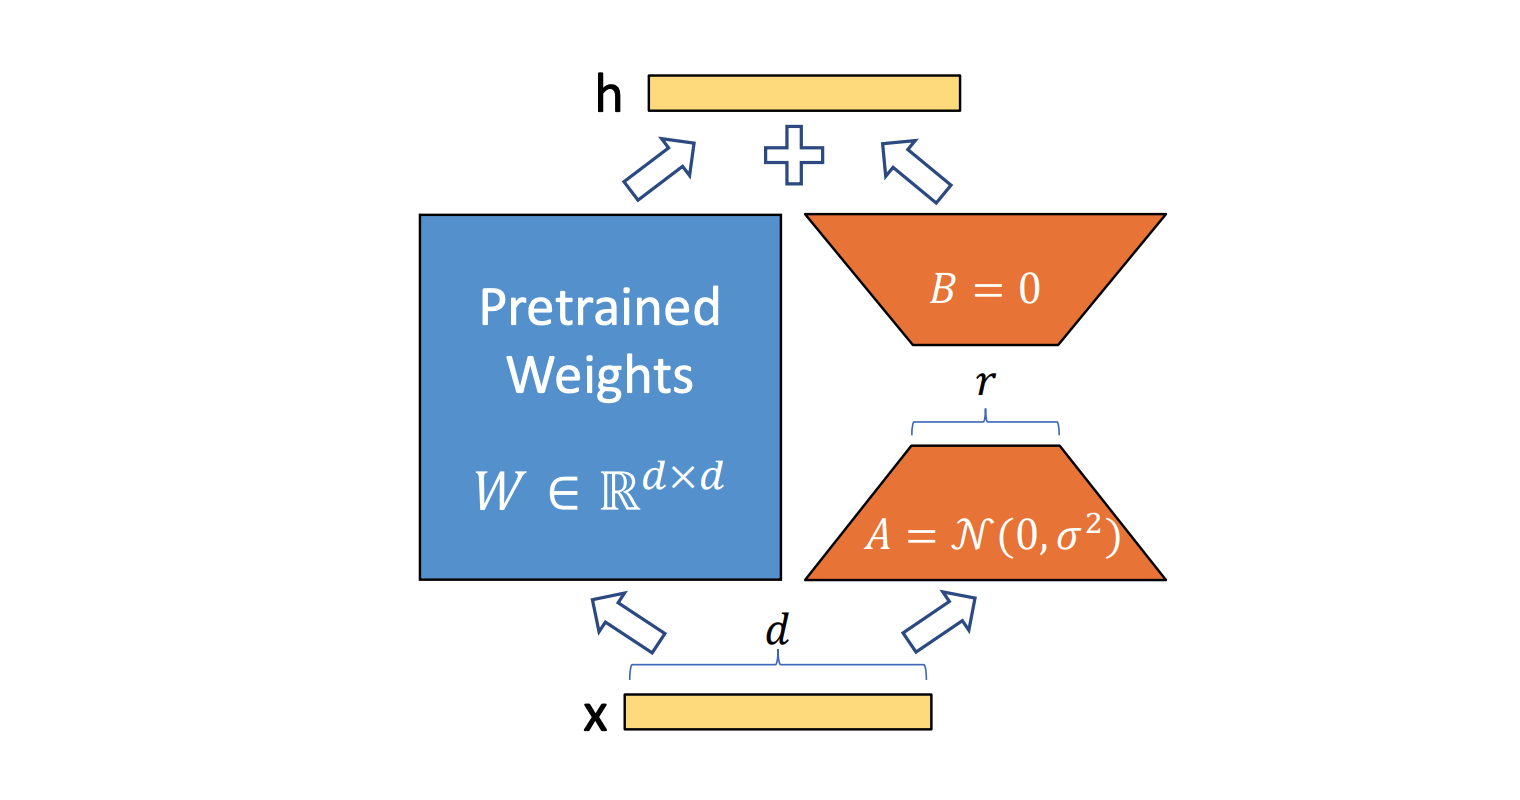
\includegraphics[width=1\textwidth]{figures/lora.png}
    \caption{\en{LoRA. Source: Adapted from Niklas Heidloff, "Efficient Fine-tuning with PEFT and LoRA" \cite{heidloff2023lora}}}
    \label{fig:lora}
\end{figure}

\subsection{Πλεονεκτήματα του \en{LoRA}}

Το \en{LoRA} παρουσιάζει σημαντικά πλεονεκτήματα, καθώς μειώνει δραστικά τον αριθμό των εκπαιδεύσιμων παραμέτρων και συνεπώς τις απαιτήσεις εκπαίδευσης, επιτρέποντας τη χρήση του ακόμη και σε συστήματα με περιορισμένους υπολογιστικούς πόρους. Παράλληλα, απαιτεί μικρότερη κατανάλωση μνήμης, γεγονός ιδιαίτερα σημαντικό για \en{edge} και κατανεμημένα περιβάλλοντα. Επιπλέον, η διαδικασία εκπαίδευσης πραγματοποιείται ταχύτερα λόγω της μειωμένης υπολογιστικής πολυπλοκότητας. Τέλος, το \en{LoRA} θεωρείται ιδιαίτερα κατάλληλο για κατανεμημένα συστήματα και δίκτυα \en{5G}/\en{6G}, χάρη στο χαμηλό κόστος υλοποίησης και την υψηλή επεκτασιμότητά του.

\section{\en{Federated Learning} και Εφαρμογές του στην Ασφάλεια Δικτύων}

\subsection{Εισαγωγή}

Η αυξανόμενη συλλογή δεδομένων στα σύγχρονα δίκτυα επικοινωνιών έχει δημιουργήσει σημαντικές ανησυχίες σχετικά με την ιδιωτικότητα, την επεκτασιμότητα και την κατανεμημένη νοημοσύνη. Στο πλαίσιο των δικτύων \en{5G} και του αναδυόμενου \en{6G}, όπου παράγονται τεράστιες ποσότητες ευαίσθητων δεδομένων από γεωγραφικά κατανεμημένες συσκευές, οι παραδοσιακές κεντρικοποιημένες προσεγγίσεις μηχανικής μάθησης παρουσιάζουν σημαντικούς περιορισμούς. Το \en{Federated Learning} έχει αναδειχθεί ως ένα υποσχόμενο εργαλείο που επιτρέπει τη συνεργατική εκπαίδευση μοντέλων χωρίς ανταλλαγή δεδομένων. Διατηρώντας τα δεδομένα τοπικά και κοινοποιώντας μόνο ενημερώσεις μοντέλων, το \en{FL} αντιμετωπίζει ζητήματα ιδιωτικότητας και επιτρέπει κατανεμημένη μάθηση μεγάλης κλίμακας \cite{kairouz2021advances,blika2025federated}.

\subsection{Ορισμός και Κίνητρο του \en{Federated Learning}}

Το \en{Federated Learning} είναι ένα κατανεμημένο πλαίσιο μηχανικής μάθησης όπου πολλοί πελάτες (\en{clients}) εκπαιδεύουν συλλογικά ένα κοινό μοντέλο υπό τον συντονισμό ενός κεντρικού εξυπηρετητή (\en{server}), διατηρώντας τα δεδομένα τους ιδιωτικά \cite{mcmahan2017communication}. Τα βασικά κίνητρα περιλαμβάνουν την προστασία της ιδιωτικότητας των δεδομένων, καθώς αυτά δεν μπορούν να κοινοποιηθούν εύκολα, την κατανεμημένη φύση των δεδομένων που βρίσκονται σε πολλές συσκευές, καθώς και τους περιορισμούς επικοινωνίας, αφού η μεταφορά μεγάλων όγκων δεδομένων είναι ιδιαίτερα δαπανηρή.

\subsection{Κεντρικοποιημένη έναντι Κατανεμημένης Μάθησης}

Η παραδοσιακή μηχανική μάθηση είναι κεντρικοποιημένη, συγκεντρώνοντας δεδομένα σε ένα σημείο, γεγονός που δημιουργεί κινδύνους ασφάλειας και ιδιωτικότητας. Αντίθετα, το \en{FL} είναι αποκεντρωμένο, διατηρώντας τα δεδομένα τοπικά και κοινοποιώντας μόνο ενημερώσεις μοντέλων. Με τον τρόπο αυτό μειώνεται ο κίνδυνος διαρροής δεδομένων, διευκολύνεται η συμμόρφωση με κανονισμούς όπως ο \en{GDPR} και επιτυγχάνεται καλύτερη επεκτασιμότητα. Ωστόσο, εισάγονται νέες προκλήσεις, όπως η ανομοιογένεια των δεδομένων και τα προβλήματα επικοινωνίας.

\subsection{Διαδικασία \en{Federated Learning}}

Η διαδικασία του \en{Federated Learning} περιλαμβάνει επαναλαμβανόμενους κύκλους συνεργασίας μεταξύ εξυπηρετητή και πελατών. Αρχικά, ο εξυπηρετητής διανέμει το αρχικό μοντέλο στους πελάτες. Στη συνέχεια, κάθε πελάτης πραγματοποιεί τοπική εκπαίδευση χρησιμοποιώντας τα δικά του δεδομένα. Έπειτα, οι ενημερώσεις αποστέλλονται πίσω στον εξυπηρετητή, ο οποίος τις συνδυάζει μέσω τεχνικών όπως το \en{Federated Averaging} \cite{mcmahan2017communication}. Η διαδικασία επαναλαμβάνεται μέχρι να επιτευχθεί σύγκλιση του μοντέλου.

\subsection{Ιδιωτικότητα και Ασφάλεια στο \en{FL}}

Το \en{Federated Learning} προσφέρει σημαντικά πλεονεκτήματα ιδιωτικότητας, καθώς τα δεδομένα δεν εγκαταλείπουν ποτέ τις τοπικές συσκευές, μειώνοντας έτσι τον κίνδυνο διαρροής. Παρ’ όλα αυτά, παραμένουν σημαντικοί κίνδυνοι, όπως οι επιθέσεις δηλητηρίασης μοντέλου, όπου κακόβουλοι πελάτες επιχειρούν να αλλοιώσουν τη συνολική συμπεριφορά του μοντέλου \cite{bhagoji2019analyzing}, καθώς και η διαρροή πληροφοριών μέσω των \en{gradients}, από τα οποία μπορεί να ανακτηθούν ευαίσθητα δεδομένα \cite{zhu2019deep}. Για την αντιμετώπιση αυτών των απειλών χρησιμοποιούνται τεχνικές όπως η Διαφορική Ιδιωτικότητα (\en{Differential Privacy}) \cite{dwork2014algorithmic} και η Ασφαλής Συνάθροιση (\en{Secure Aggregation}) \cite{bonawitz2017practical}.

\subsection{Εφαρμογές στην Ασφάλεια Δικτύων}

Το \en{Federated Learning} βρίσκει σημαντικές εφαρμογές στην ασφάλεια δικτύων, ιδιαίτερα σε συστήματα ανίχνευσης εισβολών (\en{Intrusion Detection Systems -- IDS}) και στην κατανεμημένη ανίχνευση ανωμαλιών \cite{palmos2025privacy}. Στα δίκτυα τηλεπικοινωνιών προσφέρει αυξημένη επεκτασιμότητα, επιτρέπει συνεργασία μεταξύ διαφορετικών φορέων χωρίς κοινοποίηση ευαίσθητων δεδομένων και ενισχύει τη νοημοσύνη στην περιφέρεια του δικτύου (\en{Edge Intelligence}), επιτρέποντας την άμεση επεξεργασία δεδομένων και τη λήψη αποφάσεων σε τοπικό επίπεδο.

\subsection{Πλαίσιο \en{Flower} για \en{Federated Learning}}

Το \en{Flower} είναι ένα ανοικτού κώδικα πλαίσιο για την ανάπτυξη συστημάτων \en{Federated Learning} \cite{beutel2020flower}. Η αρχιτεκτονική του βασίζεται σε έναν εξυπηρετητή (\en{server}) που συντονίζει τη διαδικασία και σε πολλούς πελάτες (\en{clients}) που εκτελούν τοπική εκπαίδευση. Μεταξύ των βασικών χαρακτηριστικών του περιλαμβάνονται η ευελιξία, η συμβατότητα με πλαίσια όπως \en{PyTorch} και \en{TensorFlow}, καθώς και η υψηλή επεκτασιμότητα. Επιπλέον, το \en{Flower} θεωρείται ιδιαίτερα κατάλληλο για την κατανεμημένη εκπαίδευση \en{LLMs}, ειδικά όταν συνδυάζεται με αποδοτικές τεχνικές όπως το \en{LoRA}.

\section{Συνδυασμός \en{LLMs}, \en{LoRA} και \en{Federated Learning}}

\subsection{Εισαγωγή}

Η ενοποίηση των Μεγάλων Γλωσσικών Μοντέλων (\en{LLMs}), τεχνικών αποδοτικής προσαρμογής παραμέτρων όπως το \en{Low-Rank Adaptation (LoRA)} και του \en{Federated Learning (FL)} αποτελεί μια πολλά υποσχόμενη κατεύθυνση για την ανάπτυξη επεκτάσιμων και φιλικών προς την ιδιωτικότητα ευφυών συστημάτων. Τα \en{LLMs} προσφέρουν ισχυρές δυνατότητες επεξεργασίας μη δομημένων δεδομένων, όπως είναι τα αρχεία καταγραφής δικτύου, αλλά συνοδεύονται από υψηλές απαιτήσεις σε υπολογιστικούς πόρους και επικοινωνία. Το \en{Federated Learning}, από την άλλη πλευρά, επιτρέπει συνεργατική εκπαίδευση χωρίς ανταλλαγή ακατέργαστων δεδομένων, καθιστώντας το κατάλληλο για τομείς όπως η κυβερνοασφάλεια. Ωστόσο, απαιτεί αποδοτικές ενημερώσεις μοντέλων ώστε να μειώνεται το κόστος επικοινωνίας \cite{mcmahan2017communication}, γεγονός που δημιουργεί μια φυσική συνέργεια με τεχνικές \en{PEFT}.

\subsection{Κίνητρο}

Τα \en{LLMs} είναι ιδιαίτερα απαιτητικά υπολογιστικά λόγω του μεγάλου αριθμού παραμέτρων που διαθέτουν, με αποτέλεσμα η πλήρης προσαρμογή τους σε περιβάλλον \en{Federated Learning} να οδηγεί σε υπερβολικό κόστος επικοινωνίας και σημαντικές απαιτήσεις σε μνήμη και επεξεργαστική ισχύ. Σε περιβάλλοντα \en{5G} και \en{6G}, όπου πολλές συσκευές διαθέτουν περιορισμένους πόρους και εύρος ζώνης, απαιτούνται αποδοτικοί μηχανισμοί εκπαίδευσης ώστε η κατανεμημένη χρήση τέτοιων μοντέλων να είναι πρακτικά εφικτή.

\subsection{Ρόλος του \en{LoRA} στο \en{Federated Learning}}

Το \en{LoRA} μειώνει δραστικά τον αριθμό των εκπαιδεύσιμων παραμέτρων, καθώς αντί για πλήρεις ενημερώσεις του μοντέλου, οι πελάτες μεταδίδουν μόνο τους πίνακες χαμηλού βαθμού που εισάγονται για την προσαρμογή \cite{hu2021lora}. Η προσέγγιση αυτή οδηγεί σε σημαντικά μειωμένο κόστος επικοινωνίας, χαμηλότερες απαιτήσεις μνήμης και ταχύτερη εκπαίδευση και συνάθροιση ενημερώσεων. Με τον τρόπο αυτό καθίσταται δυνατή η αξιοποίηση \en{LLMs} σε κατανεμημένα περιβάλλοντα με περιορισμένους πόρους.

\subsection{Ενσωμάτωση σε Επίπεδο Συστήματος}

Σε ένα συνδυαστικό σύστημα, κάθε πελάτης διατηρεί ένα τοπικό αντίγραφο του προεκπαιδευμένου \en{LLM} και εφαρμόζει προσαρμογή μέσω \en{LoRA} χρησιμοποιώντας ιδιωτικά δεδομένα. Μόνο οι παράμετροι του \en{LoRA} κοινοποιούνται στον κεντρικό εξυπηρετητή, ενώ το βασικό μοντέλο και τα δεδομένα παραμένουν τοπικά. Η διαδικασία περιλαμβάνει τη διανομή του καθολικού μοντέλου, την τοπική εκπαίδευση με \en{LoRA} και τη συνάθροιση των ενημερώσεων μέσω \en{FL}. Η αρχιτεκτονική αυτή επιτρέπει κατανεμημένη προσαρμογή μοντέλων με διατήρηση της ιδιωτικότητας και αποδοτική χρήση πόρων, καθιστώντας την ιδιαίτερα κατάλληλη για ανάλυση αρχείων καταγραφής σε μεγάλης κλίμακας τηλεπικοινωνιακά δίκτυα.

\section{Προκλήσεις και Ανοικτά Ερευνητικά Προβλήματα}

Παρά τη σημαντική πρόοδο στον συνδυασμό \en{Large Language Models (LLMs)}, \en{LoRA} και \en{Federated Learning}, εξακολουθούν να υπάρχουν αρκετές προκλήσεις και ανοικτά ερευνητικά ζητήματα που επηρεάζουν την πρακτική εφαρμογή αυτών των τεχνολογιών, ιδιαίτερα σε πολύπλοκα και μεγάλης κλίμακας περιβάλλοντα όπως τα δίκτυα \en{5G} και \en{6G}. Ένας από τους σημαντικότερους περιορισμούς είναι το επικοινωνιακό κόστος, καθώς παρότι τεχνικές όπως το \en{LoRA} μειώνουν το μέγεθος των ενημερώσεων του μοντέλου, η συχνή ανταλλαγή πληροφοριών και ο μεγάλος αριθμός συμμετεχόντων πελατών μπορούν να προκαλέσουν συμφόρηση δικτύου και αυξημένη καθυστέρηση \cite{kairouz2021advances}. Επιπλέον, τα συστήματα \en{Federated Learning} αντιμετωπίζουν συχνά προβλήματα σύγκλισης λόγω ασύγχρονων ενημερώσεων, μεταβαλλόμενης συμμετοχής των πελατών και διαφοροποιημένων συνθηκών εκπαίδευσης, γεγονός που καθιστά δύσκολη τη διασφάλιση σταθερής και αποδοτικής εκπαίδευσης. Παράλληλα, η ετερογένεια δεδομένων αποτελεί σημαντική πρόκληση, καθώς τα δεδομένα σε ομοσπονδιακά περιβάλλοντα είναι συνήθως μη ανεξάρτητα και μη ομοιόμορφα κατανεμημένα (\en{non-IID}), επηρεάζοντας αρνητικά την απόδοση των μοντέλων λόγω των διαφοροποιημένων τοπικών κατανομών μεταξύ των πελατών. Επιπρόσθετα, η επεκτασιμότητα των συστημάτων σε περιβάλλοντα \en{5G}/\en{6G} απαιτεί αποδοτική διαχείριση πόρων, προσαρμοστικές στρατηγικές επικοινωνίας και ανθεκτικό σχεδιασμό, εξαιτίας του μεγάλου αριθμού συσκευών και των συνεχώς μεταβαλλόμενων συνθηκών λειτουργίας. Τέλος, παρά την ενίσχυση της ιδιωτικότητας που προσφέρει το \en{Federated Learning}, ζητήματα όπως η διαρροή \en{gradients}, οι επιθέσεις αντιστροφής μοντέλου (\en{model inversion}) και οι προκαταλήψεις στα δεδομένα εξακολουθούν να αποτελούν σημαντικές απειλές \cite{zhu2019deep}. Παράλληλα, ζητήματα ηθικής όπως η δικαιοσύνη, η διαφάνεια και η λογοδοσία παραμένουν κρίσιμοι παράγοντες για την ασφαλή και υπεύθυνη ανάπτυξη αυτών των συστημάτων.
